\documentclass[11pt,a4paper]{article}
\usepackage{graphicx}
\usepackage{acl2021}
\usepackage{natbib}
\bibliographystyle{abbrvnat}
%%\addbibresource{lit.bib}
\usepackage{times}
\usepackage{latexsym}
\renewcommand{\UrlFont}{\ttfamily\small}

% This is not strictly necessary, and may be commented out,
% but it will improve the layout of the manuscript,
% and will typically save some space.
\usepackage{microtype}

%\aclfinalcopy % Uncomment this line for the final submission
%\def\aclpaperid{***} %  Enter the acl Paper ID here

%\setlength\titlebox{5cm}
% You can expand the titlebox if you need extra space
% to show all the authors. Please do not make the titlebox
% smaller than 5cm (the original size); we will check this
% in the camera-ready version and ask you to change it back.

\newcommand\BibTeX{B\textsc{ib}\TeX}

%\aclfinalcopy % Uncomment this line for the final submission
%\def\aclpaperid{***} %  Enter the acl Paper ID here

%\setlength\titlebox{5cm}
% You can expand the titlebox if you need extra space
% to show all the authors. Please do not make the titlebox
% smaller than 5cm (the original size); we will check this
% in the camera-ready version and ask you to change it back.

\title{Changes in Baselines of Hatespeech Detection with pretraining and Transformers}
\author{Matthias Westenfelder}


\begin{document}
\maketitle
\tableofcontents
\begin{abstract}
In this project we aim to construct a new representative baseline for Deep Neural Nets on the HatefulTwitter dataset proposed by \cite{auto_hatespeech}.
For this we implement a Transformer-based Architecture on the data and try to push the baselines proposed by the authors of the HatefulTwitter dataset.
Then we will aim to provide some evaluation of explainability and performance, also with respect to industry usecases.
\end{abstract}
 

\section{Introduction}
In their paper \cite{auto_hatespeech} propose a tweet dataset with 25.000 entries and use some basic methods to establish baselines,
especially interesting is that BoW approaches seem to have major problems distinguishing between hatespeech and offensive language since the distributions are so similar.
This might indicate that context sensitive methods are to be used. For example Transformers/BERT-models yield such a functionality.

\section{Review of \cite{auto_hatespeech}}
In this section the central question: "What did Davidson et al. actually do?" and what are the results against which we will benchmark.

\subsection{the Model}
The jist of it is the following:
They use a dataset with about 25.000 tweets. 
Then use Tidf-vectorizers on the tokens and on the POS-tags of the tweet to get a vectorized 
version of the tweet on the syntactic and on the word-level.
Then calculate a few more features based on reading-ease levels, counts of hashtags,mentions,urls and sentiment.
All these get fed into a feature selecter via logistic regression with L1-regularization ( using the liblinear solver )
for dimensionality reduction and then predictions are generated using logistic regression.

\subsection{the Results}
\cite{auto_hatespeech} claims that their final model has an overall precision of 0.91, an overall recall of 0.9 and a f1-score of 0.9.
They also claim a precision of 0.44 and recall of 0.61 (which implies a F1-score of about 0.525) on the hate class.
These claims come with an asteriks, because these numbers do not represent the performance on a test set but rather using the entire
data to train and evaluating, effectively on the trainingset. 
It is impossible to really judge how much overfitting inflates the numbers here.
What we were able to replicate is a model which achieves overall precision 0.85, recall of 0.74 and F1-score of 0.77 on a testtest of 10\% of the total data
using weighted averages.
And a precision of 0.26, recall of 0.68 and an F1-score of 0.38 on the hateclass in the testset.
Since we aim to compare the embeddings only we reran the sourcecode of Davidson with just the vectorizers on the tweet and the pos-tags.
This yielded a model with overall precision of 0.84, recall of 0.74, F1-score of 0.77
and a precision of 0.25, a recall of 0.64 and a F1-score of 0.36 on the hateclass again evaluated on 10\% of the data as a test set.
The confusion matricies can be seen in \ref{fig:feature_confusion} and \ref{fig:nofeature_confusion}.
\begin{figure}%[!ht]
  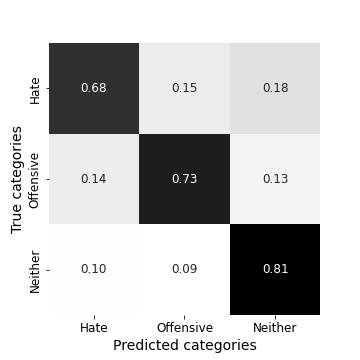
\includegraphics[width=\linewidth]{feat_confusion.jpg}
  \caption{Confusion of Model with Features}
  \label{fig:feature_confusion}
\end{figure}

\begin{figure}%[!ht]
  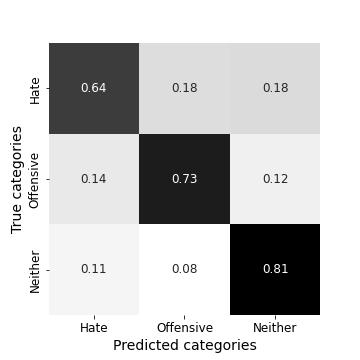
\includegraphics[width=\linewidth]{nofeat_confusion.jpg}
  \caption{Confusion of Model with no features}
  \label{fig:nofeature_confusion}
\end{figure}


\section{The Model and Implementation}
\subsection{The preprocessing}
For preprocessing of the Tweets we used the Spacy \textbf{en\_core\_web\_sm} pipeline with \textbf{EntityRuler} Component added.
Which uses identical RegEx to Davidson to identify urls mentions and excess whitespace.
Then the entire tweet is lemmatized via the Lemmatizer in the \textbf{en\_core\_web\_sm} pipeline and urls 
are replaced with a "[URL]" token, as well as mentions being replaced by a "[MENTION]" token.
The entire procedure is handeled in the function \textbf{preprocess\_tweet} in the \textit{data\_pipeline} notebook.
Here some possible improvements would be to also have a dedicated "[HASHTAG]" token as well as dealing better with elongated
versions or slightly modified versions of the same tokens. 
For example: turning "Shuuuuuuuuut upppp" or "\$hut up" into "shut up".
\subsection{The Model}
For the model we used a \textbf{distil-bert-uncased} pretrained Distilbert model with a classification head for finetuning
using the Huggingface \textbf{AutoModelForSequenceClassification} class. In addition we used the appropriate BERT-WordPiece 
tokenizer adding two custom tokens ([URL],[MENTION]) to the tokenizer.
The model gets called by the \textbf{Trainer} class via a \textbf{model\_init} method, since otherwise the classification head
weights are not connected to the \textbf{seed} parameter of the \textbf{Trainer} class.
This turns out to be a great problem to get reproducable results.
Especially in our experiments, this turned out to be a problem, since the best model we trained was not able to be replicated,
with the set seed since, we simply got lucky with the classification head weights. Which is exactly why we now use a \textbf{model\_init} method.
And also why it shouldn't be expected to get the exact weights we got once the training procedure is followed.
Which is why the Pytorch model is provided completely in the repository to make the results reproducable.
\subsection{Finetuning}
We used a custom lossfunction to mediate classimbalances.
For this we subclassed the \textbf{Trainer} class and overwrote the \textbf{compute\_loss} function with a custom function.
We use CategoricalCrossEntropy with weights for each class given by:
$$ w_i = 1 - \frac{count(class_i)}{count(data)}$$
For training we used the following Hyperparameters:
First we finetuned with: 
\begin{itemize}
    \item learning\_rate = 1e-5
    \item per\_device\_train\_batch\_size = 16
    \item per\_device\_test\_batch\_size = 16
    \item num\_train\_epochs = 5
    \item weight\_decay=0.01
    \item evalution\_strategy = "steps"
    \item eval\_steps = 500
    \item fp16 = True
    \item load\_best\_model\_at\_end = True
    \item metric\_for\_best\_model = eval\_hatef1
    \item seed = 42
\end{itemize}
Then we finetuned another pass with changes only in:
\begin{itemize}
    \item learning\_rate = 5e-6
    \item num\_train\_epochs = 2
    \item seed = 42
\end{itemize}
the rest of the unspecified hyperparameters were the default value or are paths/logging settings which aren't training
relevant and can be looked up in the \textit{train\_model} notebook.
\subsection{Results}
This yielded 
\begin{center}
\begin{tabular}{c c c c c}
class & precision & recall & f1-score & support \\
hateful & 0.58 & 0.75 & 0.66 & 134.0 \\
offensive & 0.97 & 0.96 & 0.96 & 1899.0 \\
neither & 0.96 & 0.95 & 0.96 & 446.0 \\
\end{tabular}
\end{center}

\begin{center}
\begin{tabular}{c c c c c}
metric & precision & recall & f1-score & support \\
accuracy & nan & nan & 0.94 & 2479.0 \\
macroavg & 0.84 & 0.89 & 0.86 & 2479.0 \\
weightedavg & 0.95 & 0.94 & 0.95 & 2479.0 \\
\end{tabular}
\end{center}


%\printbibliography

\bibliography{lit}

\end{document}
